\chapter{Results}\label{ch:results}

\section{Predictive and Economic Performance}\label{sec:results-performance}

Table~\ref{tab:performance_stat} reports the statistical point estimates on the
held-out test partitions. Score types and operating points follow the definitions
of Section~\ref{sec:eval}.

\begin{table}[htbp]
\centering
\small
\begin{tabular}{llccccc}
\toprule
\textbf{Dataset} & \textbf{Model} & \textbf{ROC-AUC}~$\uparrow$ & \textbf{AP}~$\uparrow$ & \textbf{Brier}~$\downarrow$ & \textbf{Bal.\ Acc.}~$\uparrow$ & \textbf{F1}~$\uparrow$ \\
\midrule
German Credit & LR & 0.815 & 0.670 & 0.153 & \textbf{0.762} & \textbf{0.653} \\
 & EBM & 0.819 & 0.619 & 0.154 & 0.736 & 0.623 \\
 & XGB & 0.814 & 0.655 & 0.160 & 0.731 & 0.620 \\
 & CatB & \textbf{0.840} & \textbf{0.709} & \textbf{0.148} & 0.743 & 0.639 \\
\midrule
Taiwan & LR & 0.705 & 0.481 & 0.145 & 0.673 & 0.491 \\
 & EBM & \textbf{0.777} & 0.539 & 0.138 & 0.709 & 0.532 \\
 & XGB & 0.775 & \textbf{0.544} & \textbf{0.137} & 0.707 & 0.531 \\
 & CatB & 0.775 & 0.543 & \textbf{0.137} & \textbf{0.715} & \textbf{0.540} \\
\midrule
Home Credit & LR & 0.744 & 0.225 & 0.069 & 0.680 & 0.259 \\
 & EBM & \textbf{0.756} & \textbf{0.241} & \textbf{0.068} & \textbf{0.691} & \textbf{0.270} \\
 & XGB & 0.754 & 0.239 & \textbf{0.068} & 0.688 & 0.260 \\
 & CatB & 0.754 & 0.239 & \textbf{0.068} & 0.688 & 0.266 \\
\midrule
Lending Club & LR & 0.708 & 0.377 & 0.145 & 0.650 & 0.425 \\
 & EBM & 0.721 & 0.394 & 0.143 & 0.661 & 0.437 \\
 & XGB & 0.728 & 0.404 & \textbf{0.142} & 0.665 & 0.441 \\
 & CatB & \textbf{0.729} & \textbf{0.405} & \textbf{0.142} & \textbf{0.666} & \textbf{0.443} \\
\bottomrule
\end{tabular}
\caption[Statistical performance by dataset and model]{Test-set point estimates of
statistical performance by dataset and model. Balanced accuracy and $F_1$ use the
frozen base-rate threshold.}
\label{tab:performance_stat}
\end{table}

On German Credit, the point ordering varies by metric: CatBoost has the highest ROC-AUC and AP and the lowest Brier score, whereas logistic regression has the highest
balanced accuracy and $F_1$. On Taiwan, the EBM, XGBoost and CatBoost lie within $0.002$
ROC-AUC of one another, while the remaining metrics do not reproduce that ordering:
XGBoost has the highest AP, CatBoost the highest displayed balanced accuracy and $F_1$, and
XGBoost and CatBoost are level at the displayed Brier score; logistic regression trails
the three non-linear configurations by about $0.07$ ROC-AUC. On Home Credit, the EBM has
the best or tied-best displayed estimate for all five statistical metrics. On Lending Club, XGBoost and CatBoost lead the EBM across the
reported point estimates, while logistic regression is further behind.

After isotonic calibration, the within-dataset spread between the four Brier scores is
at most $0.012$. Raw and calibrated values are compared in
Table~\ref{tab:brier_calibration}.

Figure~\ref{fig:emp_levels} reports the economic point estimates. EMP summarises
the expected maximum excess profit supported by a model's test-set score ranking
relative to the lend-to-all reference policy, under the fixed economic assumptions
of Section~\ref{sec:eval}. The potential principal of each case is normalised to
one monetary unit, and cases enter equally, so observed loan amounts do not affect
the measure. An EMP of $2.480\%$ therefore corresponds to $0.0248$ principal units
per scored case---or, illustratively, EUR~24.80 for a standardised principal of
EUR~1{,}000. It denotes neither an improvement in predictive accuracy nor realised
portfolio profit.

EMP integrates the maximum profit attained at potentially different cut-offs across
the assumed uncertainty in loss given default. It is therefore an upper-bound
evaluation measure rather than the profit realised at one frozen deployment
threshold. EMP levels are compared only
within a dataset because class prevalence and economic parameters differ across
datasets. Because hyperparameters were selected on validation ROC-AUC, the results concern discrimination-selected rather
than EMP-optimised configurations.


\begin{figure}[htbp]
\centering
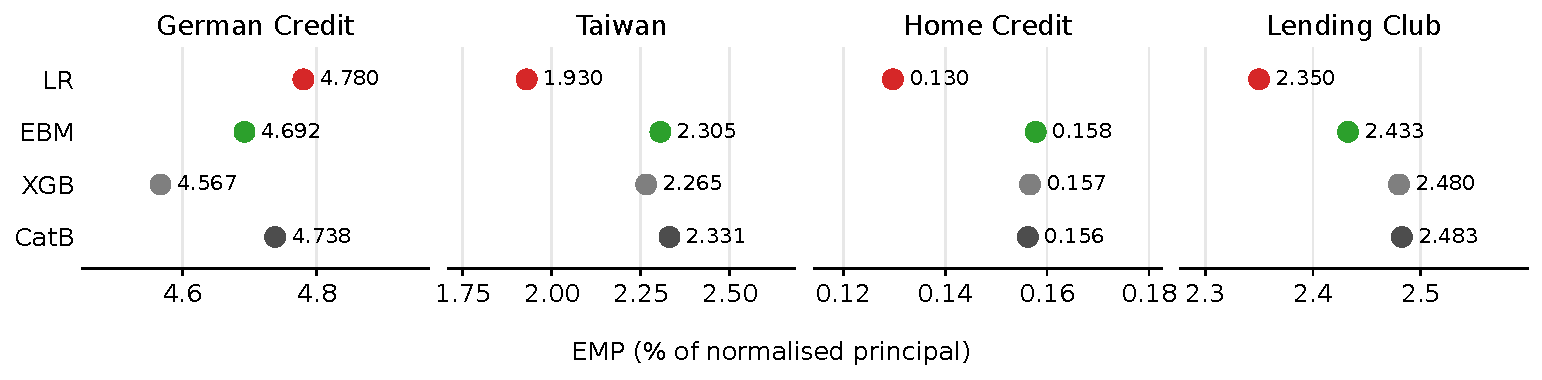
\includegraphics[width=\textwidth]{img/fig_emp_levels.pdf}
\caption[Economic performance by dataset and model]{Test-set EMP by dataset and model}
\label{fig:emp_levels}
\end{figure}

EMP among the three non-linear configurations spans $0.065$ percentage points on Taiwan
and $0.002$ on Home Credit. On Lending Club, XGBoost and CatBoost reach $2.480\%$ and
$2.483\%$, compared with $2.433\%$ for the EBM and $2.350\%$ for logistic regression, so
the ensemble--EBM differences are $0.047$ and $0.050$ percentage points of normalised
principal. German Credit shows a different point ordering, with logistic regression
reaching the highest EMP at $4.780\%$. 


\paragraph{Paired model comparisons.}
The point estimates establish the observed ordering, but not how sensitive the
between-model differences are to the composition of the held-out sample. The paired
bootstrap therefore evaluates whether the direction of the central cross-group
contrasts remains resolved under test-case resampling. Differences are defined as
$\Delta=a-b$, where $a$ is LR or the EBM and $b$ is XGBoost or CatBoost. An interval
entirely above zero indicates a higher numerical value for the intrinsically
interpretable model; one entirely below zero indicates a higher value for the
ensemble. An interval containing zero leaves the direction unresolved under this
procedure. Excluding zero does not establish practical relevance. The intervals are
unadjusted for multiplicity and conditional on the split, fitted pipelines and observed
class counts. Figure~\ref{fig:cross_group_differences} displays the four contrasts that
compare LR or the EBM directly with each boosted ensemble.

\begin{figure}[!htbp]
\centering
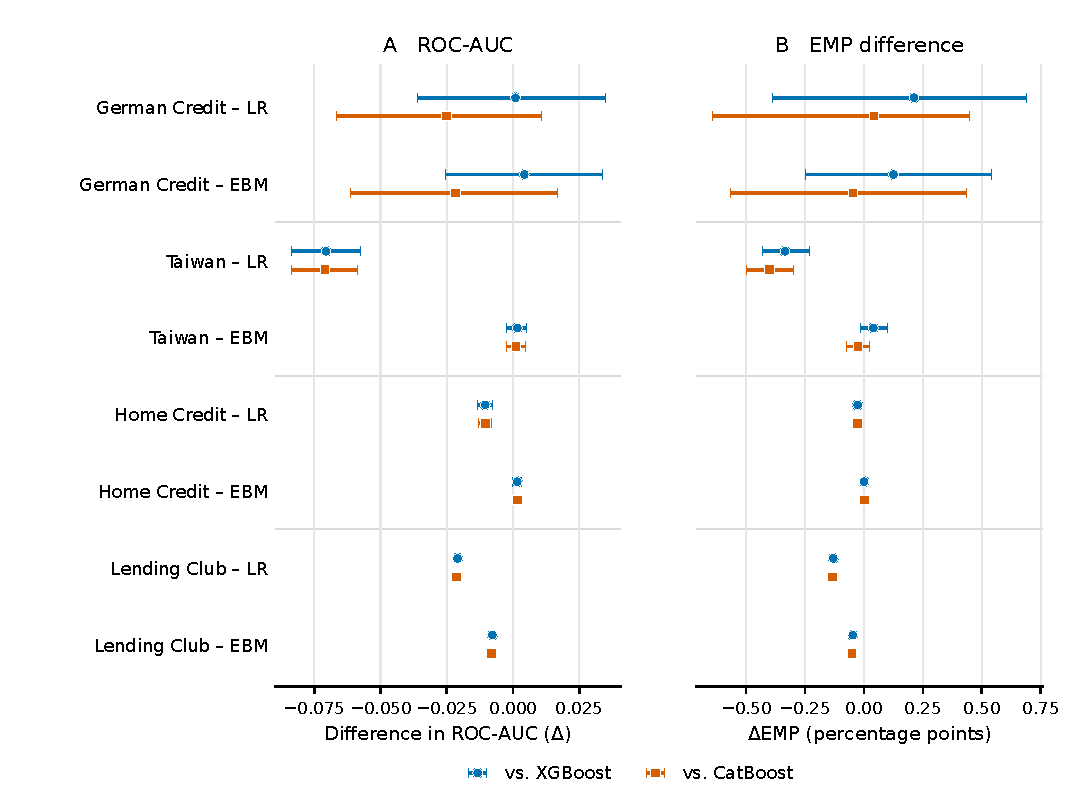
\includegraphics[width=0.90\textwidth]{img/fig_cross_group_differences.pdf}
\caption[Cross-group differences in ROC-AUC and EMP]{Cross-group differences in
ROC-AUC and EMP with unadjusted 95\% paired percentile-bootstrap intervals. Positive
values favour LR or the EBM; negative values favour the boosted ensemble.}
\label{fig:cross_group_differences}
\end{figure}

On German Credit, none of the EBM--ensemble intervals resolve a direction. On Taiwan,
all four EBM--ensemble intervals for ROC-AUC and EMP contain zero, so the procedure
resolves no direction there either. On Home Credit, the EBM is approximately level with
or slightly ahead of the ensembles: its ROC-AUC interval against CatBoost excludes zero,
whereas the interval against XGBoost narrowly contains it, and neither EMP interval
resolves a direction. In contrast, on Lending Club all four EBM--ensemble
intervals for ROC-AUC and EMP lie entirely below zero, so both ensembles lead the EBM on
both metrics. For logistic regression, the corresponding ROC-AUC and EMP intervals
against both ensembles also lie below zero on Taiwan and Lending Club.

The complete paired results for all six model pairs and all six metrics are reported in
Tables~\ref{tab:delta_pairs}, \ref{tab:delta_pairs_ap_brier} and
\ref{tab:delta_pairs_threshold}. German Credit produces the widest paired intervals,
consistent with its test partition of only $200$ observations; no paired interval for
any of the six metrics excludes zero there.

\section{Supplementary Evidence from Attribution Rankings}\label{sec:results-explainability}

The following analyses concern two properties of the global source-feature attribution
rankings: their stability under case resampling and their agreement across models. They
are not a comprehensive measurement of explainability or explanation quality.

\subsection{Case-Sampling Stability}\label{sec:results-stability}

For each pipeline, top-ten membership is the mean bootstrap inclusion frequency of the
ten features leading its original global ranking: a value of one means that these ten
features remain in the top ten in every resample. Rank-interval width is the mean width,
measured in rank positions, of their 95\% bootstrap rank intervals; smaller values
indicate less movement within the ranking.

Table~\ref{tab:shap_stability} reports these quantities conditional on the fitted
model--explainer pipelines. Mean top-ten membership ranges from $0.929$ to $1.000$, while
mean rank-interval width ranges from $0.20$ to $2.10$ positions.

The point estimates show no consistent stability advantage for logistic regression or
the EBM over XGBoost and CatBoost. This comparison is descriptive because no intervals
were computed for differences between pipelines; the reported rank intervals quantify
feature-rank variation within a pipeline, not uncertainty in between-pipeline
differences.

Absolute stability levels are not interpreted comparatively across datasets.
German Credit uses only $200$ explained test cases, whereas $2{,}000$ cases are
used for each larger dataset. In addition, the top ten account for $50.0\%$ of
the $20$ available source features on German Credit and $43.5\%$ of the $23$ on
Taiwan, compared with $13.9\%$ of the $72$ on Home Credit and $16.1\%$ of the
$62$ on Lending Club. Top-ten membership is therefore a less selective criterion
in the lower-dimensional datasets, additionally restricting direct comparison of
absolute stability levels.

\begin{table}[htbp]
\centering
\small
\begin{tabular}{llcc}
\toprule
\textbf{Dataset} & \textbf{Model} & \textbf{Top-10 membership}~$\uparrow$ & \textbf{Rank-interval width}~$\downarrow$ \\
\midrule
German Credit & LR & 1.000 & 2.00 \\
 & EBM & 0.929 & 2.10 \\
 & XGB & 1.000 & 1.40 \\
 & CatB & 0.998 & 1.40 \\
\midrule
Taiwan & LR & 0.988 & 0.90 \\
 & EBM & 1.000 & 0.80 \\
 & XGB & 1.000 & 0.20 \\
 & CatB & 0.980 & 1.10 \\
\midrule
Home Credit & LR & 1.000 & 0.40 \\
 & EBM & 0.997 & 0.70 \\
 & XGB & 0.965 & 0.80 \\
 & CatB & 0.964 & 0.40 \\
\midrule
Lending Club & LR & 0.989 & 0.70 \\
 & EBM & 1.000 & 0.60 \\
 & XGB & 0.998 & 0.60 \\
 & CatB & 0.999 & 0.40 \\
\bottomrule
\end{tabular}
\caption[Global attribution-rank stability under case resampling]{Case-sampling
stability of the ten features leading each original global ranking over $1{,}000$
bootstrap resamples.}
\label{tab:shap_stability}
\end{table}

\FloatBarrier

\subsection{Cross-Model Agreement}

Table~\ref{tab:cross_model_agreement} reports two complementary forms of agreement.
Jaccard is the size of the intersection of two top-ten sets divided by the size of their
union, so it ranges from zero for no shared feature to one for identical sets and is not
the share of features on which two pipelines agree. Mean pairwise Jaccard provides a
compact descriptive summary of top-ten overlap across the six model pairs. Spearman
correlation instead compares the ordering of the complete source-feature rankings and is
reported as a descriptive point estimate without an interval.

\begin{table}[htbp]
\centering
\fontsize{8.5pt}{10pt}\selectfont
\setlength{\tabcolsep}{3pt}
\begin{tabular}{@{}lccccccc@{}}
\toprule
 & \textbf{Jaccard [95\% bootstrap int.]} & \multicolumn{6}{c}{\textbf{Pairwise Spearman}~$\uparrow$} \\
\cmidrule(lr){2-2}\cmidrule(lr){3-8}
\textbf{Dataset} & \textbf{Mean pairwise} & \shortstack{LR\\EBM} & \shortstack{LR\\XGB} & \shortstack{LR\\CatB} & \shortstack{EBM\\XGB} & \shortstack{EBM\\CatB} & \shortstack{XGB\\CatB} \\
\midrule
German Credit & 0.717 [0.717, 0.747] & 0.89 & 0.82 & 0.88 & 0.89 & 0.91 & 0.95 \\
Taiwan        & 0.532 [0.486, 0.532] & 0.27 & 0.19 & 0.17 & 0.94 & 0.87 & 0.94 \\
Home Credit   & 0.649 [0.649, 0.696] & 0.92 & 0.88 & 0.89 & 0.97 & 0.97 & 0.99 \\
Lending Club  & 0.696 [0.696, 0.696] & 0.87 & 0.81 & 0.86 & 0.89 & 0.95 & 0.92 \\
\bottomrule
\end{tabular}
\caption[Cross-model agreement on which features matter]{Agreement between
model--explainer pipelines: mean pairwise top-ten Jaccard with its 95\% bootstrap
interval and pairwise Spearman correlations of the complete rankings.}
\label{tab:cross_model_agreement}
\end{table}

Mean pairwise top-ten Jaccard ranges from $0.532$ on Taiwan to $0.717$ on German Credit.
These raw levels are not read as a cross-dataset ordering, because the overlap expected
by chance increases as the number of available source features decreases. The degenerate
Lending Club interval reflects an unchanged mean overlap at the reported precision across
the central resamples. It does not imply an absence of uncertainty under retraining or
population change.

Agreement in the complete rankings is strongest among the three non-linear
configurations. Across datasets, the EBM's Spearman correlations with XGBoost and
CatBoost range from $0.87$ to $0.97$. Logistic regression remains broadly aligned on
German Credit, Home Credit and Lending Club but diverges on Taiwan, where its
correlations with the other models range from $0.17$ to $0.27$.

Table~\ref{tab:top_features} locates that divergence. All four Taiwan pipelines rank
\texttt{PAY\_0} first, but logistic regression fills the remaining top-five positions
with three bill-amount columns and \texttt{MARRIAGE}, whereas the three non-linear
configurations share \texttt{LIMIT\_BAL} and further repayment-status terms. The
divergence is therefore concentrated below the leading feature rather than spread
across the ranking.

\section{Sensitivity Analyses}

\subsection{Training-Set Size Sensitivity}\label{sec:size}

Figure~\ref{fig:learning_curves} reports test ROC-AUC and across-refit top-ten Jaccard
at the realised training sizes on Home Credit and Lending Club. Each value is the mean
of three refits under one manually specified configuration frozen across all sample sizes, each
refit drawing its own stratified subsample of that size from the training partition;
only the displayed grid points were run, so no behaviour between them is estimated.

\begin{figure}[htbp]
\centering
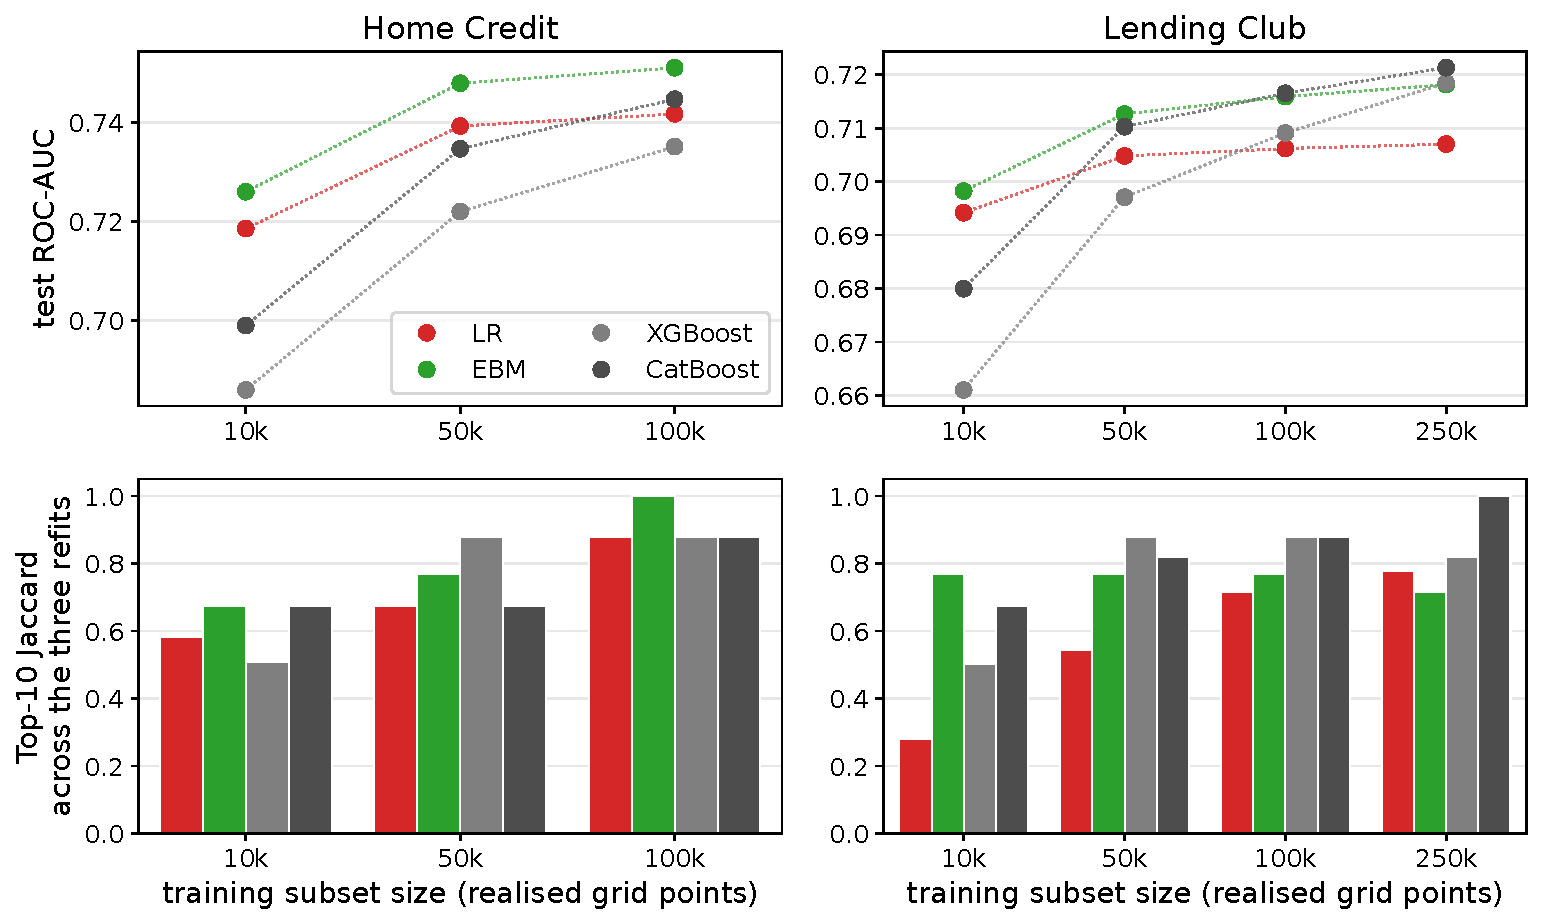
\includegraphics[width=\textwidth]{img/fig_learning_curves.pdf}
\caption[Training-size sensitivity of ROC-AUC and attribution-rank overlap]{Mean test
ROC-AUC (top) and mean pairwise top-ten Jaccard (bottom) across three refits at each
realised training size under fixed configurations.}
\label{fig:learning_curves}
\end{figure}

ROC-AUC rises across the realised grid for all four frozen configurations. XGBoost and
CatBoost show the largest numerical endpoint gains on both datasets, between $+0.041$
and $+0.057$, logistic regression the smallest, $+0.013$ and $+0.023$, and the EBM lies
between them. The maximum-minus-minimum ROC-AUC spread across the four configurations
narrows from $0.040$ to $0.016$ on Home Credit and from $0.037$ to $0.014$ on Lending
Club. The EBM remains above logistic regression at every realised size, while the two
ensembles close their initial deficits and have slightly higher endpoint estimates
on Lending Club.

These changes across the realised grid describe the training-size sensitivity of the
frozen configurations, not the general sample efficiency of optimally tuned model
families. The configurations differ
in capacity, only three repetitions were run per point, no interval was computed for
differences in change, and neither grid reaches the full headline training partition.
Across-refit top-ten Jaccard generally increases with training size, although not
monotonically for every configuration. On Home Credit, the endpoint values range from
approximately $0.88$ to $1.00$ at $100{,}000$ observations, compared with $0.50$ to
$0.67$ at $10{,}000$. On Lending Club, logistic regression rises from approximately
$0.28$ to $0.78$ and CatBoost from $0.67$ to $1.00$, whereas the EBM ends slightly below
its earlier values and XGBoost declines after reaching about $0.88$ at the intermediate
grid points.


\FloatBarrier

\subsection{Out-of-Time Evaluation}\label{sec:temporal-results}

\providecommand{\dbunit}{\setlength{\unitlength}{1mm}}
\providecommand{\dumbbell}[3]{%
  \raisebox{-0.4ex}{%
    \begingroup\dbunit
    \begin{picture}(42,2)(0,0)
      \linethickness{0.7mm}\put(#1,1){\line(1,0){#3}}
      \put(#1,1){\circle*{2}}
      \linethickness{0.25mm}\put(#2,1){\circle{2}}
    \end{picture}%
    \endgroup
  }%
}
\providecommand{\dbaxis}{%
  \raisebox{-0.4ex}{%
    \begingroup\dbunit
    \begin{picture}(42,5)(0,0)
      \linethickness{0.15mm}\put(0,5){\line(1,0){42}}
      \multiput(6.3,3.8)(10.5,0){4}{\line(0,1){1.2}}
      \put(6.3,0){\makebox(0,0)[b]{\scriptsize 0.70}}
      \put(16.8,0){\makebox(0,0)[b]{\scriptsize 0.71}}
      \put(27.3,0){\makebox(0,0)[b]{\scriptsize 0.72}}
      \put(37.8,0){\makebox(0,0)[b]{\scriptsize 0.73}}
    \end{picture}%
    \endgroup
  }%
}

Lending Club is the only dataset with an origination timestamp. The out-of-time run fits
on loans issued through 2014, tunes on 2015, refits through 2015 and evaluates the
resolved 2016--2018 cohort. Table~\ref{tab:oot_perf} compares it with the random-split
headline estimates.

\begin{table}[htbp]
\centering
\small
\begin{tabular}{@{}lccc@{}}
\toprule
\textbf{Model} & \textbf{ROC-AUC}~{\footnotesize($\bullet$~OOT, $\circ$~random)} & \shortstack{$\boldsymbol{\Delta}$~\textbf{ROC-AUC}\\{\footnotesize(OOT$-$random)}} & \shortstack{\textbf{EMP}\\{\footnotesize(\% of principal)}} \\
\midrule
LR       & \dumbbell{4.79}{14.19}{8.40}  & $-0.009$ & 1.97 \\
EBM      & \dumbbell{17.41}{27.99}{9.58} & $-0.010$ & 2.04 \\
XGBoost  & \dumbbell{22.23}{36.15}{12.92} & $-0.013$ & \textbf{2.06} \\
CatBoost & \dumbbell{22.40}{36.53}{13.13} & $-0.013$ & \textbf{2.06} \\
 & \dbaxis & & \\
\bottomrule
\end{tabular}
\caption[Lending Club out-of-time evaluation]{Random-split and out-of-time performance
on Lending Club, read off a common horizontal scale: the filled and hollow points denote
the out-of-time and random-split ROC-AUC, respectively, and their connecting segment
represents the descriptive difference $\Delta=\text{OOT}-\text{random}$. EMP is that of
the temporal run, under its own frozen economic configuration.}
\label{tab:oot_perf}
\end{table}

The out-of-time ROC-AUC estimates are between $0.009$ and $0.013$ below the corresponding
random-split estimates, while the broad point ordering---the two ensembles ahead of the
EBM and the EBM ahead of logistic regression---is retained.

Because the two ROC-AUC estimates arise from different training windows and
evaluation populations, $\Delta$ is a descriptive contrast between validation
designs rather than a paired estimate of temporal degradation.

On unrounded values, the EBM trails XGBoost and CatBoost by $0.0046$ and $0.0048$
ROC-AUC, respectively---approximately $0.005$ in both comparisons, against approximately
$0.008$ under the random split. No interval was computed for either design contrast or
for this difference of differences, so the numerical narrowing is descriptive.

Within the temporal run, the broad economic ordering is also retained: XGBoost and
CatBoost reach an EMP of $2.06\%$ of normalised principal, compared with $2.04\%$ for the
EBM and $1.97\%$ for logistic regression. These levels are comparable only within the
temporal run, because its class prior and return parameter are re-derived from the
temporal training window. The analysis concerns resolved loans only. Because
resolution-based selection becomes substantially stronger in the later vintages, the
observed out-of-time differences cannot be attributed to temporal population change
alone.
